%----------------------------------------------------------
\chapter*{ВВЕДЕНИЕ}\label{chap.introduction}
\addcontentsline{toc}{chapter}{ВВЕДЕНИЕ}
% =========================================================================== %
% ----------------------------- ОСНОВНЫЕ ПУНКТЫ ----------------------------- %
% 1. Описание задач, в которых нужно всякое навороченное математическое ПО
% 2. Примеры наовороченного математического ПО
%   2.1. Почему просто математического ПО не всегда достаточно?
%   2.2. Упомянуть про задачи, у которых одна и та же постановка, но разные 
%         параметры
% 3. Примеры ПО, которое рассчитано на многократное решение задач, автоматизи-
%    рующее их решение (Scientific workflow, hallo?)
%   3.1. Использование графов при описании логики решения в системах научных
%        расчётов
%   3.2. Неудобства в описании данных
%   3.3. Визуальное программирование
% 4. Итог: нужно ПО, где есть какая-то абстракция над обрабатываемыми данными,
%    где они конкретизируются непосредственно в реализациях этапов алгоритма.
% 5. Enter GBSE and comsdk
%    5.1. А чем оно, собсна, так привлекательно?
%    5.2. Сказать про НОВЫХ пользователей (Р А С Ш И Р Я Е М О С Т Ь)
% 6. Сравнение GBSE и DFD
% =========================================================================== %
Современные научно-технические исследования зачастую включают в себя задачи, при решении которых требуется большое количество вычислений, для которых задействуются большие вычислительные мощности. К таким задачам относятся, например, задачи анализа, определения характеристик материалов или технических объектов, моделирования сложных динамических процессов. Как правило, для решения подобных задач применяется или разрабатывается специализированное программное обеспечение (\glsxtrshort{ПО}).

Среди прочих применяются программные продукты, предоставляющие пользователю формальный язык описания математических выражений и его интерпретатор, выполняющий необходимые вычисления на машине пользователя. К таким системам относятся, например, Mathcad. Также стоит отметить системы специализирующиеся на символьной алгебре, такие, как Maple~\cite{CharMaple1983} и Wolfram Mathematica. В настоящее время данные программные комплексы поддерживают решение задач из различных областей математики, включающих в себя теорию графов, теорию множеств и~т.д, предоставляют инструменты визуализации и анализа результатов. Все они позволяют выполнять математическое моделирование, в том числе, сложных технических объектов. При всех их преимуществах необходимость формулировать математические постановки решаемых задач (т.е.~формировать математические модели, составлять системы уравнений и~т.д.) остаётся за пользователем. Зачастую требуется решать множество задач с схожей постановкой, но с различными входными параметрами. Такая необходимость, например, возникает при решении задач оптимизации, где критерием является некоторая характеристика, получаемая в результате решения задачи анализа. Следовательно, целесообразны автоматизированные средства решения типовых задач анализа и моделирования.

Данные средства относятся к специализированному \glsxtrshort{ПО}, а потому при их разработке требуются глубокие познания в предметной области. Кроме того, важно, чтобы создаваемая кодовая база была рассчитана на дальнейшую поддержку, что предъявляет соответствующие требования к структуре исходного кода и документации. Таким образом, целесообразно применение некоторых средств, позволяющих организовать разработку программного обеспечения для решения задач моделирования и анализа и повысить его поддерживаемость.

В наши дни популярность приобретает применение т.н. научных систем управления потоком задач (англ.~scientific workflow systems). Они предоставляют средства организации этапов решения вычислительной задачи и управления вычислительными ресурсами. Процесс работы с подобными системами состоит из 4 основных этапов:
\begin{enumerate}[1)]
  \item составление описания операций обработки данных и зависимостей между ними;
  \item распределение процессов обработки данных по вычислительным ресурсам;
  \item выполнение обработки данных;
  \item сбор и анализ результатов и статистики~\cite{DeelmanWorkflow2009}.
\end{enumerate}

Примерами подобных систем могут служить Pegasus~\cite{DeelmanPegasus2016}, Kepler~\cite{AltintasKepler2004} и pSeven~\cite{NazarenkoDFM2015}. Помимо инструментов загрузки пользовательских реализаций этапов решения задачи они, как правило, представляют библиотеку типовых действий и преобразований, таких, как считывание данных и их сохранение в файлы одного из поддерживаемых форматов, операции со строками, работы с базами данных, и~т.д. Кроме того, некоторые из них имеют средства интеграции с другими системами моделирования и анализа, что позволяет задействововать их при расчётах. На рисунке~\ref{fig:intro.keplerScreenshot} изображён пример описания некоторого процесса в системе Kepler.

\begin{figure}[!ht]
  \centering
  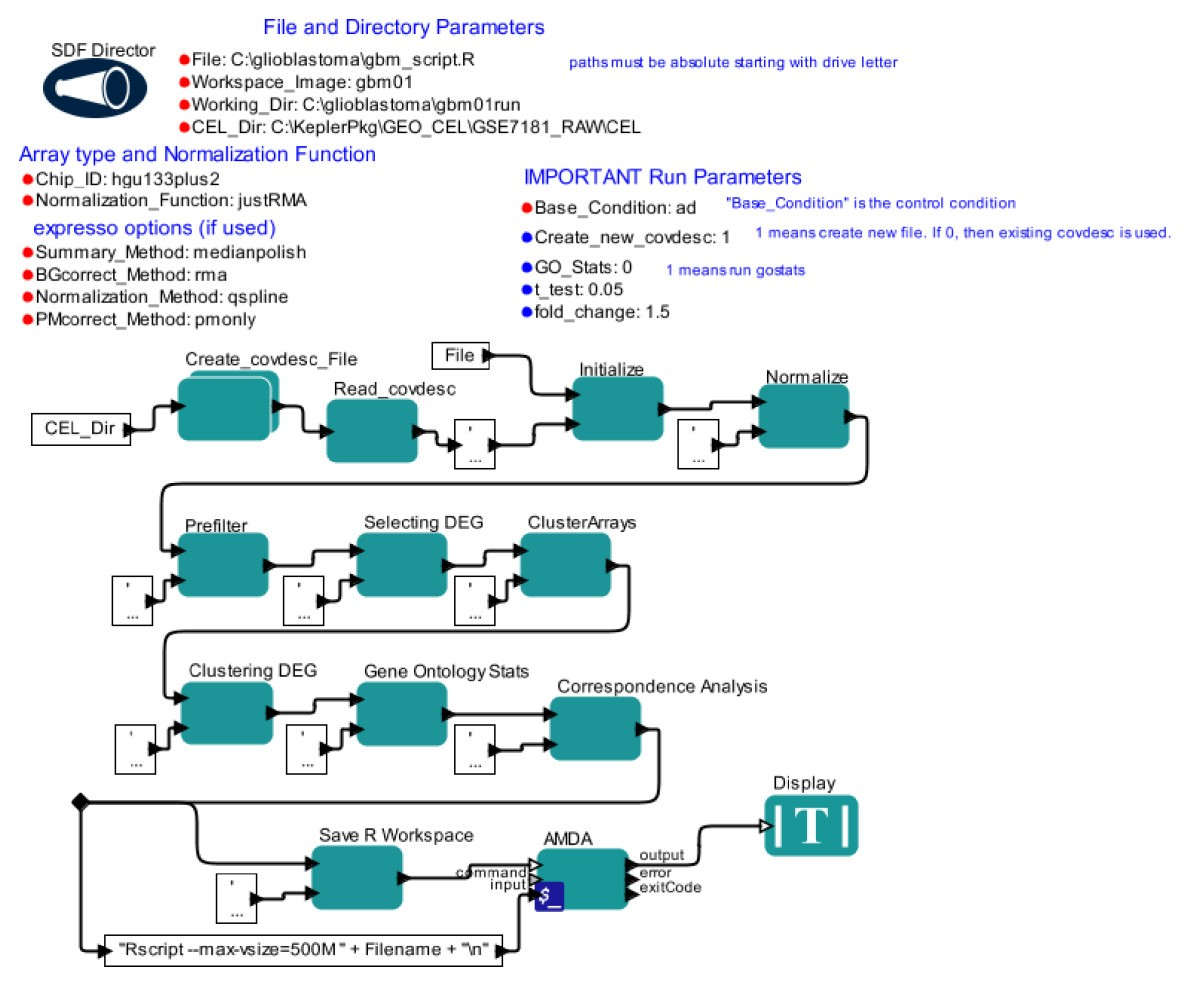
\includegraphics[height=0.45\textheight]{figures/screenshot.KeplerWorkflow.jpg}
  \caption{Описание процесса обработки данных в системе Kepler}
  \label{fig:intro.keplerScreenshot}
\end{figure}

Кроме того, для облегчения процесса разработки трудоёмкого ПО существуют т.н. платформы малокодовой разработки (англ.~low-code development platforms, \glsxtrshort{LCPD})~\cite{DiRuscio2022}. В них, подобно системам управления потоком задач, логика разрабатываемого программного продукта описывается при помощи некоторого формального языка или с использованием графического редактора. От системы к системе подход к описаниям варьируется. Может применяться структурный подход, описывающий шаги алгоритма, или предметно-ориентированный, при котором описываются взаимодействующие сущности. Некоторые системы позволяют по созданному описанию генерировать готовые компоненты будущего программного продукта. Так платформа Codebots реализует предметно-ориентированный подход и по составленным UML-диаграммам взаимодействующих сущностей позволяет генерировать \glsxtrshort{API}, \glsxtrshort{JSON}-схемы данных и документацию~\cite{DiRuscio2022}. Тем не менее при реализации сложных вычислительных методов целесообразнее использовать структурный подход.

Одной из ключевых особенностей описанных технологических решений является выделение операций обработки данных в отдельные программные модули (функции, подпрограммы, скрипты). Как правило, при создании описаний алгоритмов в них используется следующий подход. Поскольку известно, что выходные данные одного программного модуля могут являться входными для одного или нескольких других модулей, можно сказать, что между ними формируются зависимости по входным и выходным данным. Тогда возможно составить такой ориентированный граф, описывающий общую логику алгоритма, в котором узлами являются операции обработки данных, а рёбрами -- пути данных. Такой подход получил название ``диаграммы потоков данных'' (англ.~Dataflow Diagram, \glsxtrshort{DFD}). На рисунке~\ref{fig:exampleDataflow} приведён пример такого ориентированного графа, описывающего процесс вычисления среднего арифметического и среднего геометрического двух массивов вещественных чисел.
\begin{figure}
  \centering
  \includegraphics[width=\textwidth]{figures/example.dataflow.png}
  \caption{Пример диаграммы потоков данных}
  \label{fig:exampleDataflow}
\end{figure}

При известных входных и выходных данных каждого модуля они могут создаваться независимо друг от друга~\cite{DanilovPar2011}. Возникает возможность распределения задач создания отдельных программных модулей между разработчиками. Таким образом, уменьшается объём работы по написанию исходных кодов, приходящийся на одного исследователя. Это, в свою очередь, облегчает отладку и написание документации, что положительно сказывается на общем качестве реализуемого ПО.

В приведённом выше подходе существует необходимость явно описывать входные и выходные данные каждого процесса обработки. При этом на начальных этапах проектирования не всегда требуемые данные могут быть полность определены в силу недостатка представлений о программной реализации тех или иных этапов. Таким образом, в некоторых случаях может быть целесообразен такой подход к построению описания логики реализуемого решения, что в нём не указываются конкретные обрабатываемые данные. Последовательность выполнения отдельных этапов в таком случае должна задаваться явно. В предпринимательстве и управлении проектами подобный подход широко распространён и реализован в сетевых графиках. Сетевой график представляет собой ориентированный граф, в котором вершины -- это события или состояния проекта, а рёбра -- это работы. В работе~\cite{SokolovPershin2018} рассматривается применение идеи переходов между состояниями при описании логики вычислительных алгоритмов. Описанный подход получил название graph-based software engineering (\glsxtrshort{GBSE}). Кроме того в указанной работе описана реализация GBSE в библиотеке comsdk для языка C++.

Таким образом, объектом разработки является программный каркас для реализации сложных вычислительных методов comsdk. Целью разработки является создание новых программных средств для описания и представления графовых моделей сложных вычислительных методов и их обхода. Для достижения цели были поставлены следующие задачи:
\begin{enumerate}[1)]
  \item провести аналитический обзор источников по теме ``Системы для реализации сложных вычислительных методов'';
  \item провести сравнение рассматриваемой разработки с аналогом;
  \item cформировать требования к алгоритму интерпретации графовых описаний, составленных по методологии GBSE;
  \item спроектировать структуры данных для описания и представления графовых моделей и их элементов в программном каркасе comsdk;
  \item разработать алгоритм обхода графовых моделей с использованием спроектированных структур данных;
  \item реализовать разработанные алгоритмы и структуры данных на языке С++.
\end{enumerate}